% Report of results from Ramsay simulation experiment
% David Lawrence Miller
% d.l.miller@bath.ac.uk

% Started : 8th April 2009

\documentclass[a4paper,10pt]{amsart}

% Load some packages
\usepackage{times, amsmath, amssymb, amsfonts, url, natbib, bm, rotating,multirow,graphicx}
\usepackage[margin=1in]{geometry}

% top matter
\title{Smoothing over irregular shapes using the Schwarz-Christoffel transform}
\author{David Lawrence Miller}
\email{d.l.miller@bath.ac.uk}
\address{Mathematical Sciences, University of Bath, Bath, United Kingdom}

% Shortcuts
% Probability
\newcommand{\prob}[1]{\mathbb{P}\left[ #1 \right]}
% Hovitz-Thompson
\newcommand{\HT}{\hat{\tau}_{HT}}
% Schwarz-Christoffel
\newcommand{\sch}{Schwarz-Christoffel }
% fprime
\newcommand{\fprime}{f^\prime(z)}
% figure reference command
\newcommand{\fig}[1]{\emph{fig.} (\ref{#1})}
% figure reference command (start of sentance
\newcommand{\Fig}[1]{\emph{Fig.} (\ref{#1})}
% equation reference command
\newcommand{\eqn}[1]{\emph{eqn.} (\ref{#1})}
% phi inverse
\newcommand{\phiinv}{\phi^{-1}}
% use other phi
\newcommand{\ophi}{\phi}
\renewcommand{\phi}{\varphi}




\begin{document}

% The abstract
\begin{abstract}
Following on from looking at the Ramsay horseshoe, other polygon mappings are simulated from and transformed with the \sch transform. [ADD CONCLUSION HERE]
\end{abstract}


% New theorem for theorems
\newtheorem{thm}{Theorem}[section]

%New theorem for definitions
\newtheorem{defn}{Definition}[section]

\maketitle



\section{Looking at other domains}

Given the relative success of using the \sch transform on the Ramsay horseshoe, and the relative failure of using it on the alternate Ramsay horseshoe, more conclusive evidence is needed to investigate the properties of the transform and its utility to smoothing over complex regions.





\section{General setup}

For all of the examples below the function \texttt{mvnorm} from the \textsf{R} package \texttt{MASS} was used to generate a  multivariate Normal surface over the region in question. This was then discretized over a 50x50 grid. A 500 replicate simulation experiment was then run at two noise levels ($\sigma^2=0.02$, $\sigma^2=0.005$) and two sample sizes (1000, 500.) For each replicate we fit a smooth of thin plate regression splines, the soap film smoother of \cite{soap} and finally thin plate regression splines on the \sch transformed domain. The transformation was performed by the \textit{SC Toolbox for MATLAB} and models were fit using \texttt{mgcv} in \textsf{R}. We then compared the results from each model by calculating the mean squared error over a prediction grid over the region.

\section{Example 1}

We begin with an example from \cite{miller09}. The shape (shown in \fig{fig9-disk-real}) does not include any kind of peninsula, such as that in the Ramsay horseshoe, this is a deliberate of the performance of the \sch transform method and the soap film smoother in such situations. 

The shape was morphed to both the unit disk and the rectangle to see if this made a difference to the fit. For the rectangular mapping, vertices chosen (somewhat arbitrarily) to map to those of the rectangle were 1, 6, 8 and 9 (see \fig{fig9-numbered}.)

For the soap film smoother a 7 by 7 grid of which 17 inside knots were used and 

\begin{figure}[tbp]
\centering
% trim order l b r t
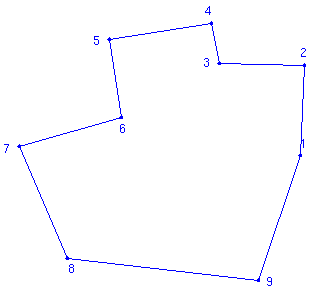
\includegraphics[width=2in]{figs-otherdomains/fig9-numbered.png} \\
\caption{Vertex numbering for the first example.}
\label{fig9-numbered}
% generated by Matlab
\end{figure}



\begin{figure}[p]
\centering
% trim order l b r t
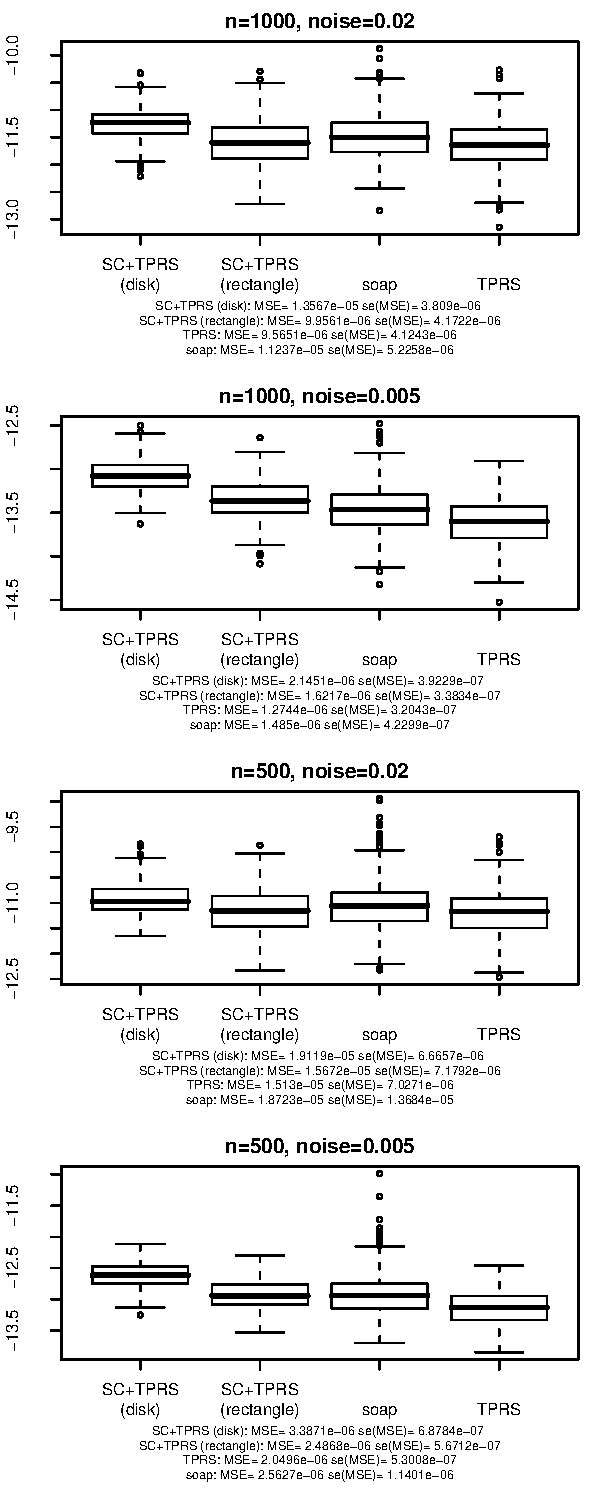
\includegraphics[width=4in]{figs-otherdomains/fig9-boxplot.pdf} \\
\caption{Boxplot of mean squared error per prediction point over 500 replicates for example 1 on the log-scale. Non-log-scaled measurements below.}
\label{fig9-boxplots}
% generated by fig9test/makeboxplots.R
\end{figure}

\Fig{fig9-disk-real} shows an example fit for the three methods along with the true surface when the region is deformed to the unit disk. \Fig{fig9-rect-real} shows an analogous diagram for the rectangular domain transform. The results of the simulations are summarized in the boxplots in \fig{fig9-boxplots}.

\begin{figure}[tbp]
\centering
% trim order l b r t
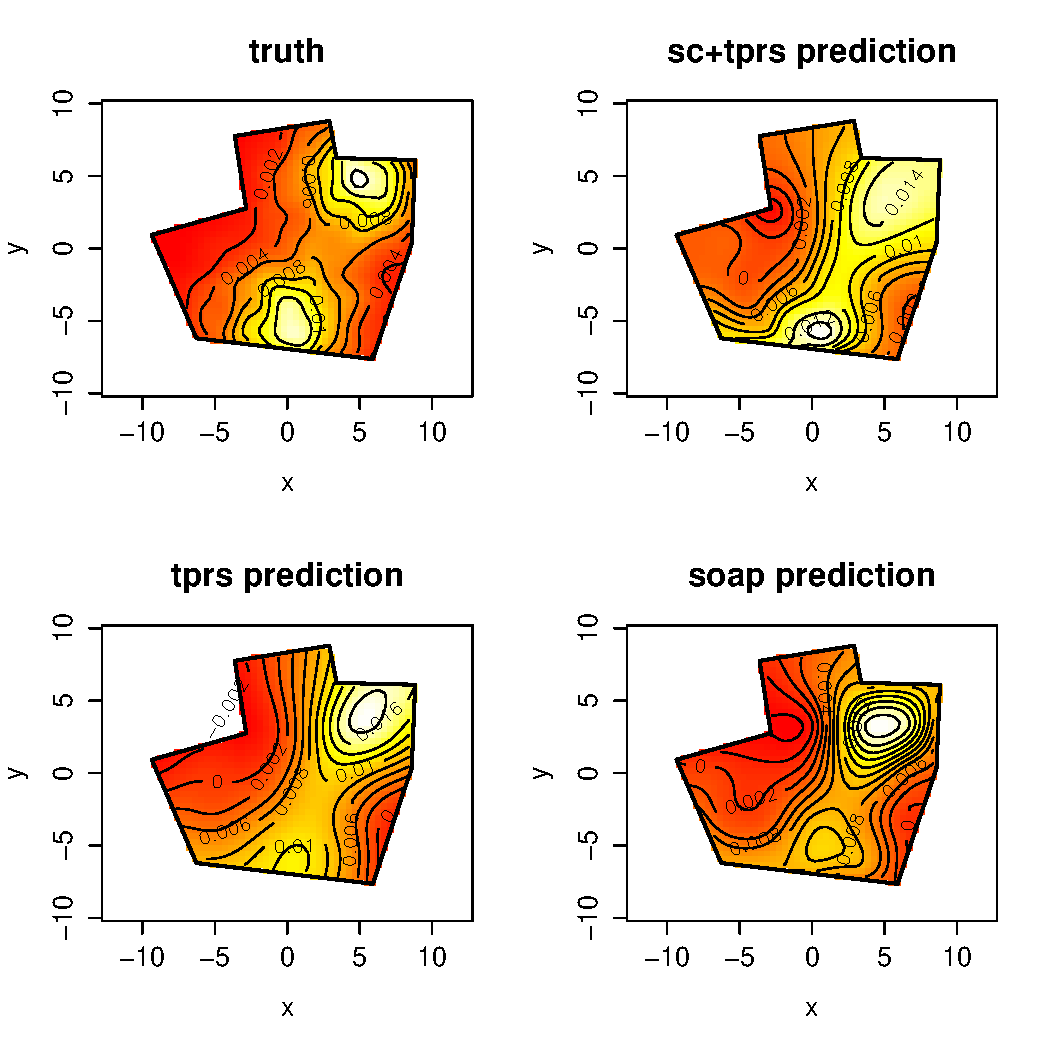
\includegraphics[width=3in]{figs-otherdomains/fig9-disk-real.pdf} \\
\caption{Truth and fits from one realization of the first example when it was transformed to the disk. Here the sample size was 500 and the noise level was set to 0.02.}
\label{fig9-disk-real}
% generated by fig9test/fit.irregular.R
\end{figure}

From this we can see that the thin plate regression splines appear to do very well for all cases, having the smallest for each configuration. The MSEs become closer as the sample size drops.

Looking at \fig{fig9-disk-real} and \fig{fig9-rect-real} we can see that the \sch transform method seems to want to join the two high density points in the surface. This is presumably due to the ``bunching-up'' of space due to the transform. Indeed, this effect can be seen in \fig{fig9-rect-bunching} and \fig{fig9-disk-bunching}.


\begin{figure}[tbp]
\centering
% trim order l b r t
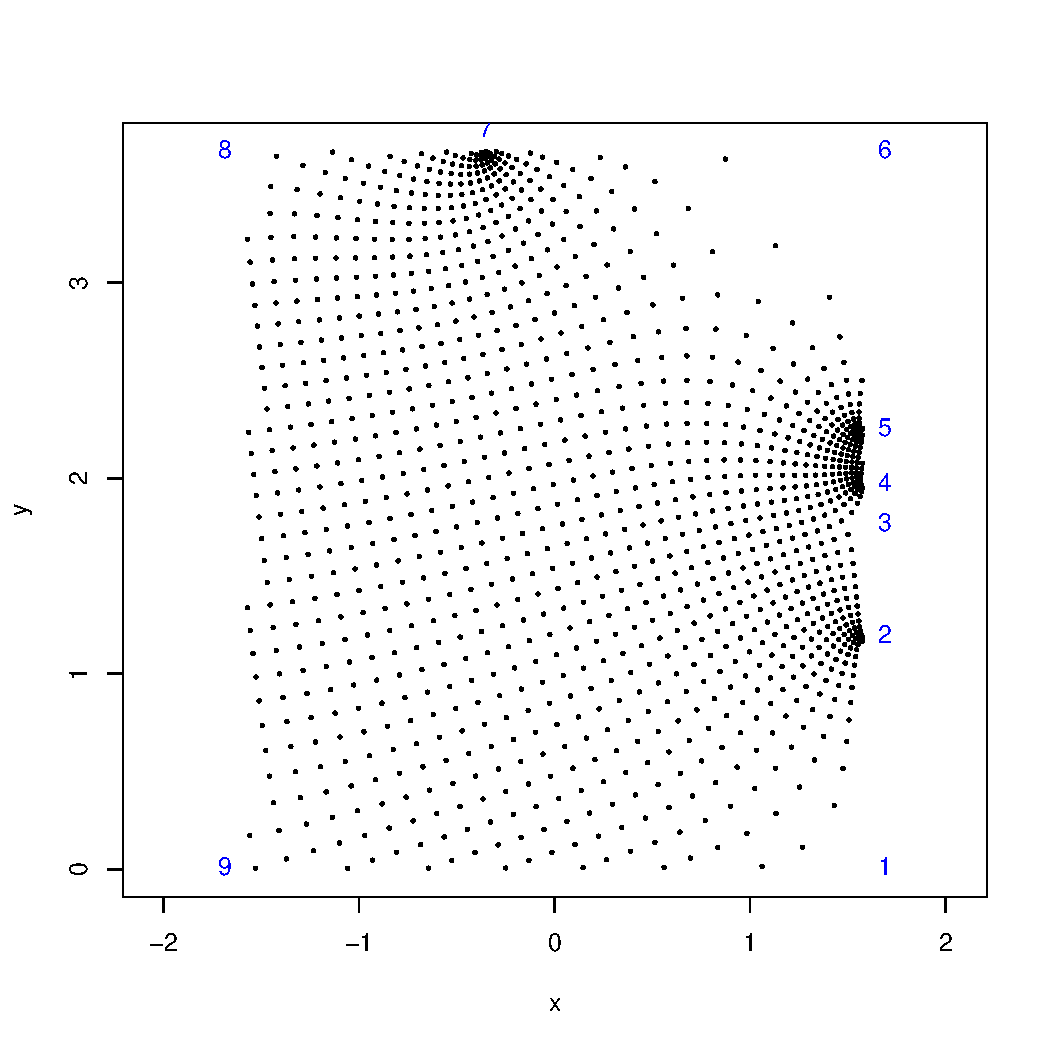
\includegraphics[width=2.5in]{figs-otherdomains/fig9-pointplot-rect.pdf} \\
\caption{A plot of how a regular grid over the original domain is transformed using the \sch rectangular mapping. Numbers give vertices from \fig{fig9-numbered} under the mapping.}
\label{fig9-rect-bunching}
% generated by figs-otherdomains/fig9-pointmap.R 
\end{figure}


\begin{figure}[tbp]
\centering
% trim order l b r t
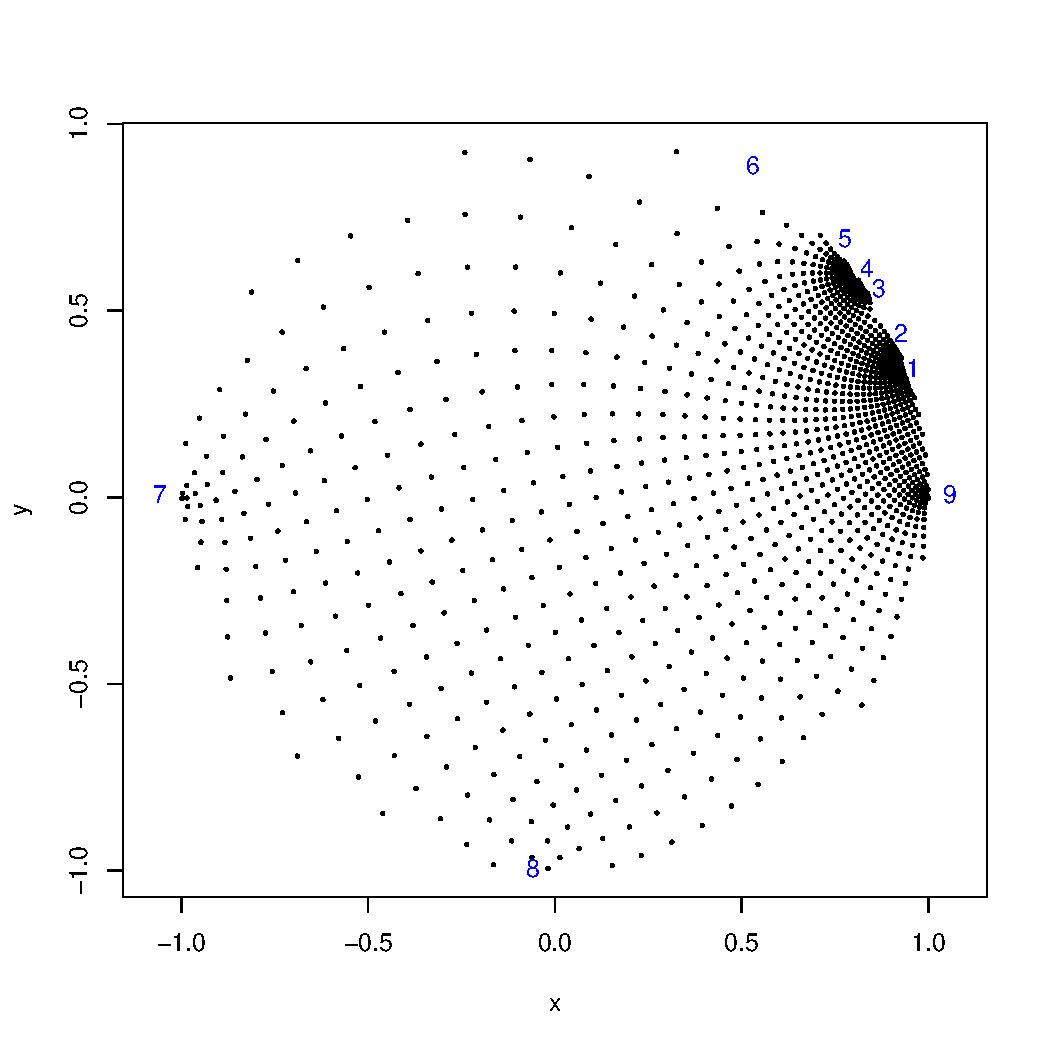
\includegraphics[width=2.5in]{figs-otherdomains/fig9-pointplot-disk.pdf} \\
\caption{A plot of how a regular grid over the original domain is transformed using the \sch unit disk mapping. Numbers give vertices from \fig{fig9-numbered} under the mapping.}
\label{fig9-disk-bunching}
% generated by figs-otherdomains/fig9-pointmap.R 
\end{figure}


\begin{figure}[tbp]
\centering
% trim order l b r t
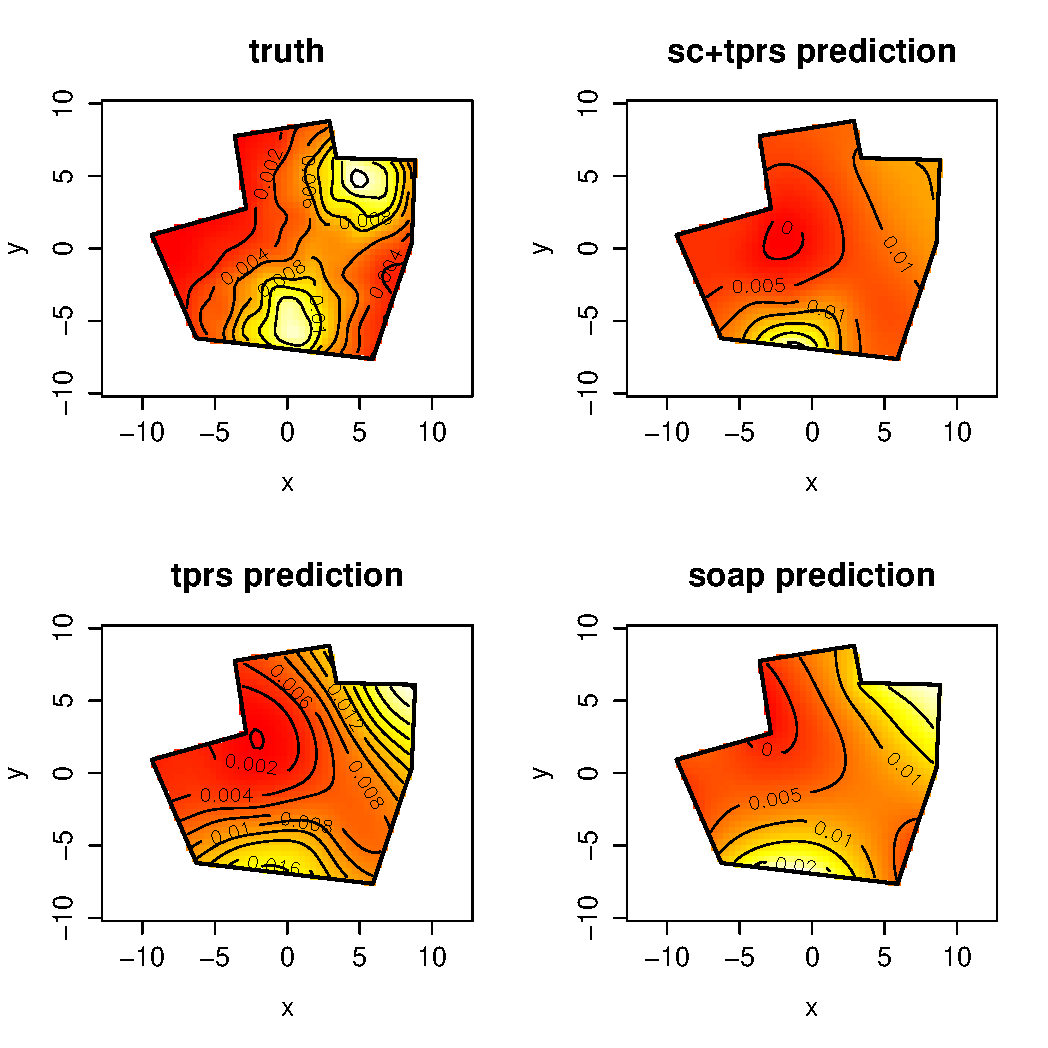
\includegraphics[width=3in]{figs-otherdomains/fig9-rect-real.pdf} \\
\caption{Truth and fits from one realization when there was a sample size of 500 and the noise level was set to 0.02 when the rectangular mapping was used. }
\label{fig9-rect-real}
% generated by fig9test/fit.irregular.R
\end{figure}




%%%%%%%%%%%%%%%%%%%%%%%%%%%%%%%%%%%%%%%%%%%%%%%%%%%%%%%%
\section{Example 2}

The second example here is supposed to simulate the kind of domain that is common in surveys of marine animals, where there is some kind of peninsula in the domain. \Fig{wigglytop-numbered} shows the region in question. For this example a mapping to the rectangle was used with the vertices 1, 2, 3, and 18 used in order to try to squash the irregularities in the top of the domain. Other vertex combinations (as well as the CRDT method) were used but showed no particular advantage over the combination presented here\footnote{Indeed, some caused MATLAB to crash.}.




For the soap film, several knot configurations were tried, the best one was to have 20 boundary knots (for the cyclic spline) and a 7 by 7 grid of knots over the domain (of which 25 were inside the domain.) 






\begin{figure}
\centering
% trim order l b r t
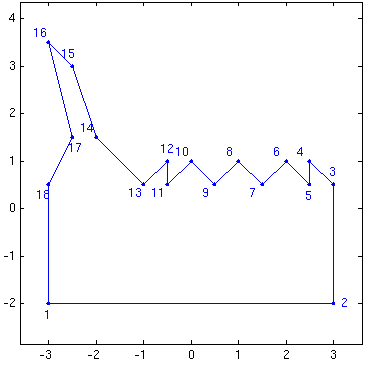
\includegraphics[width=2in]{figs-otherdomains/wigglytop-numbered.png} \\
\caption{Vertex numbering for the second example.}
\label{wigglytop-numbered}
% generated by Matlab
\end{figure}




% boxplot
\begin{figure}[p]
\centering
% trim order l b r t
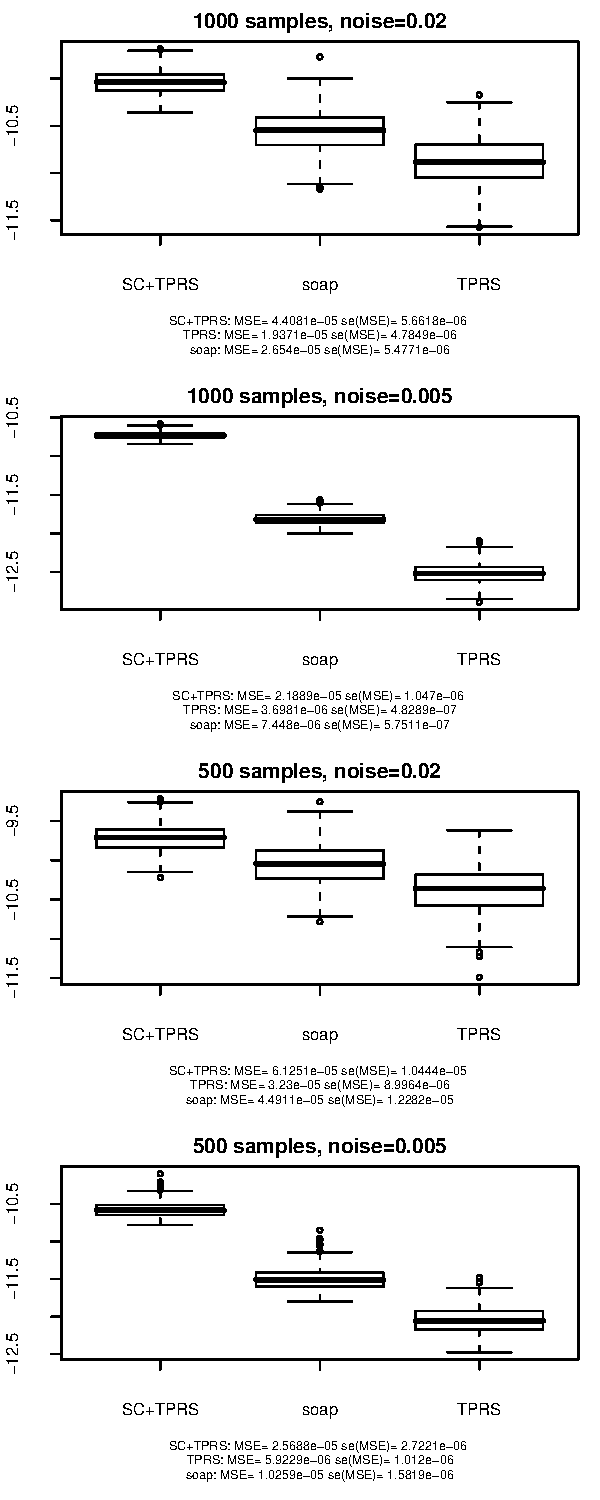
\includegraphics[width=4in]{figs-otherdomains/wigglytop-boxplot.pdf} \\
\caption{Boxplot of mean squared error per prediction point over 500 replicates for the rectangle mapping for example 2. }
\label{wigglytop-boxplots}
% generated by makeboxplots.R
\end{figure}


% realization
\begin{figure}
\centering
% trim order l b r t
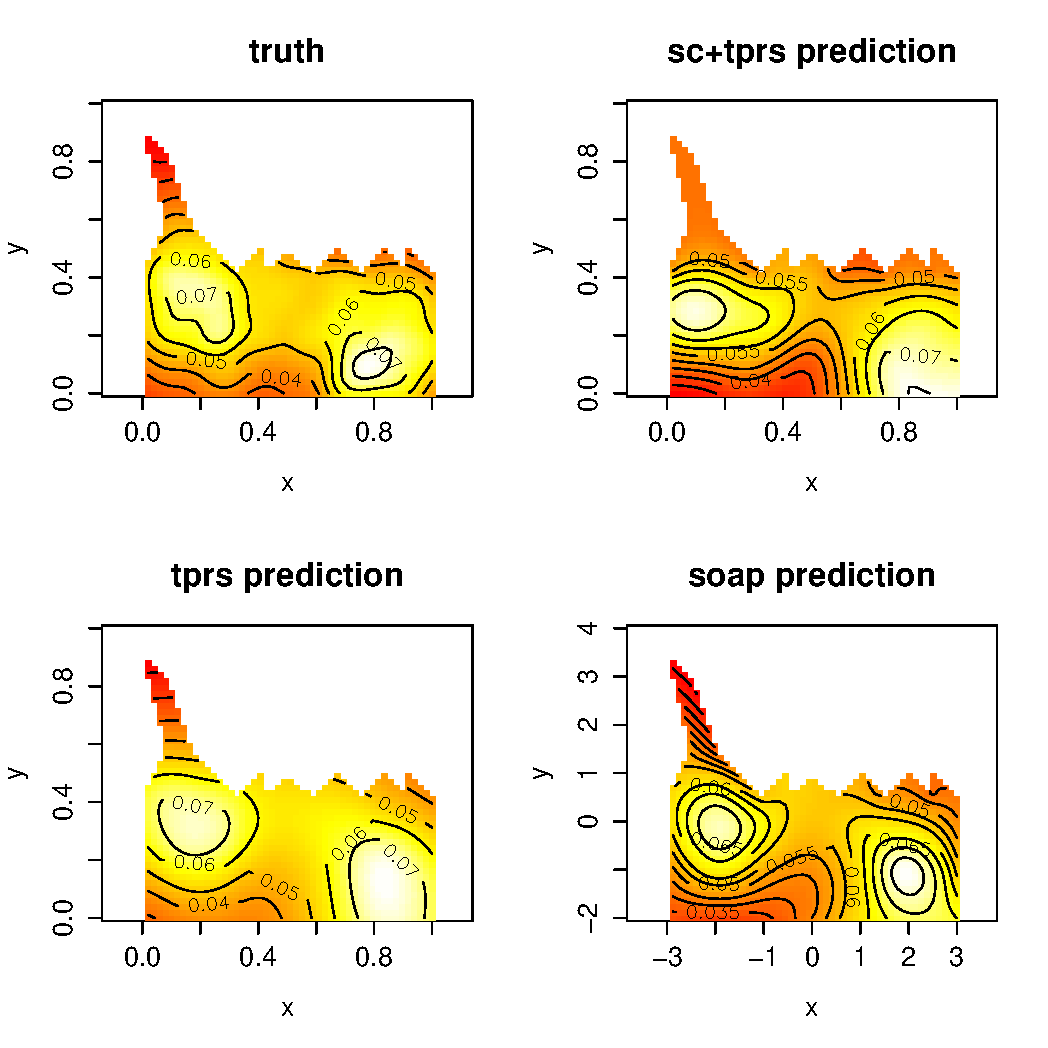
\includegraphics[width=3in]{figs-otherdomains/wigglytop-real.pdf} \\
\caption{Truth and fits from one realization when there was a sample size of 500 and the noise level was set to 0.02 when the rectangular mapping was used for example 2. }
\label{wigglytop-real}
% generated by wigglytop fit.irregular.R
\end{figure}





%%%%%%%%%%%%%%%%%%%%%%%%%%%%%%%%%%%%%%%%%%%%%%%%%%%%%%%%%%%%%%%%%%%%%%
\section{Example 3}

We repeated the procedure for another polygon with two peninsulae, shown in \fig{wigglytop2dia}. Initially, a transform using \texttt{rectmap} was used, but this failed to converge, so \texttt{crrectmap} was used.

\begin{figure}
\centering
% trim order l b r t
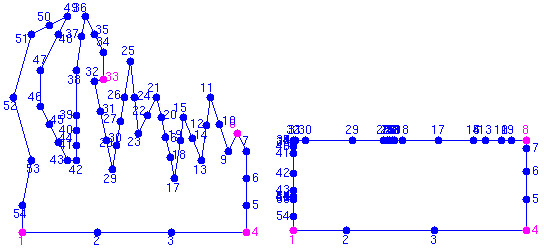
\includegraphics[width=2in]{figs-otherdomains/wigglytop2-numbered.png} \\
\caption{CRDT pic. EXPLAIN}
\label{wigglytop2-numbered}
% generated by Matlab
\end{figure}

% boxplot
\begin{figure}[p]
\centering
% trim order l b r t
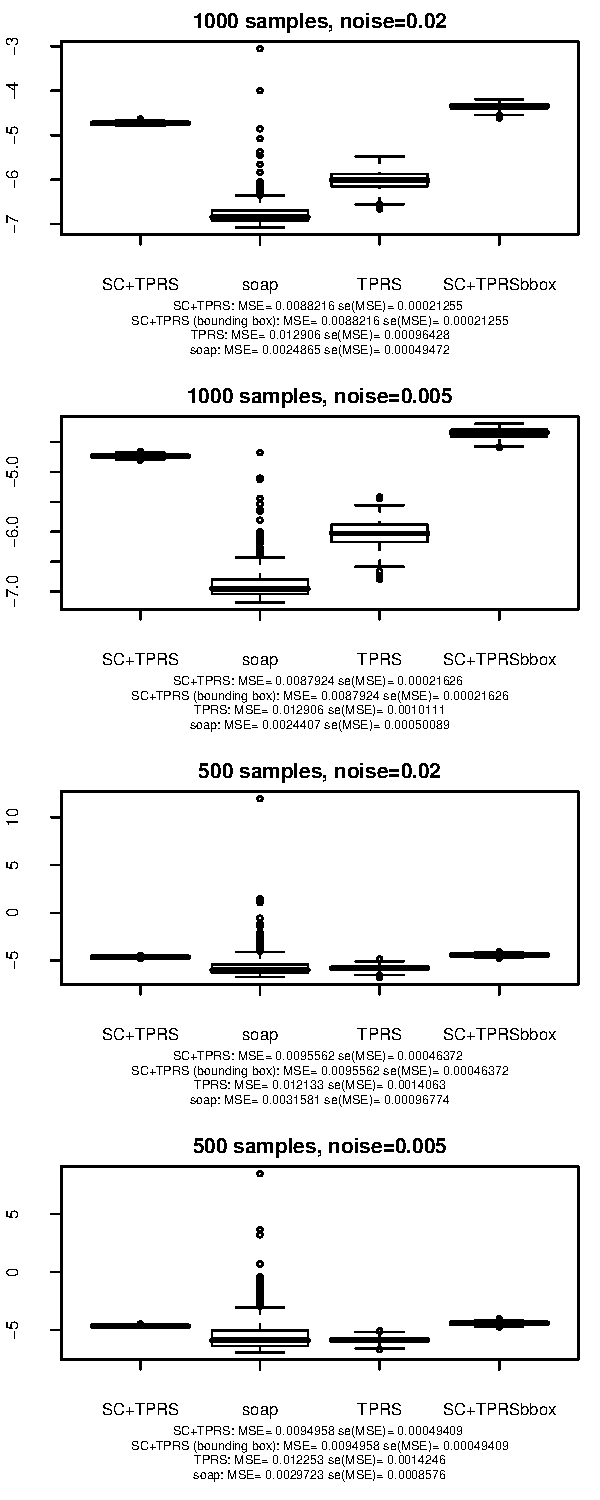
\includegraphics[width=3in]{figs-otherdomains/wigglytop2-boxplot.pdf} \\
\caption{Boxplot of mean squared error per prediction point over 500 replicates for the rectangle mapping for example 3. }
\label{wigglytop2-boxplots}
% generated by makeboxplots.R
\end{figure}


% realization
\begin{figure}
\centering
% trim order l b r t
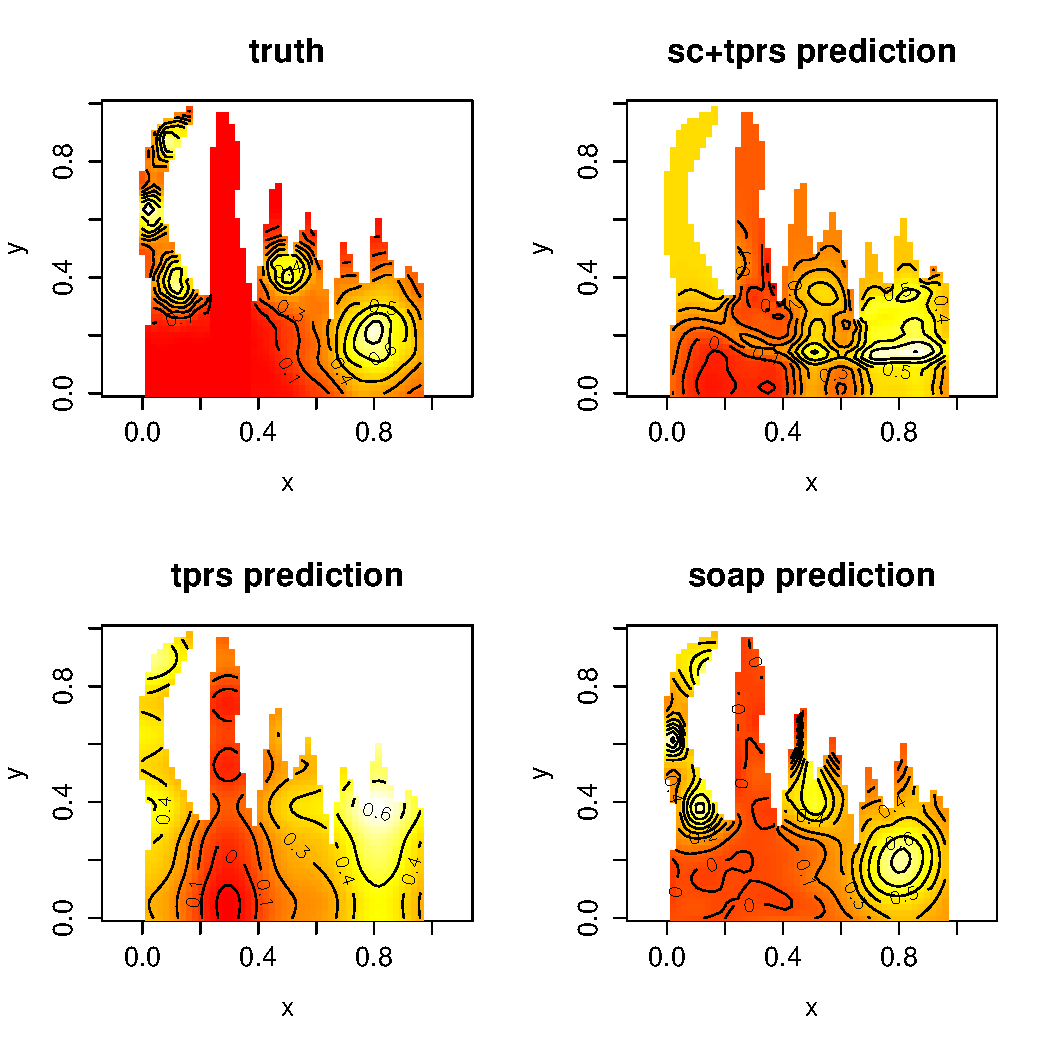
\includegraphics[width=3in]{figs-otherdomains/wigglytop2-real.pdf} \\
\caption{Truth and fits from one realization when there was a sample size of 500 and the noise level was set to 0.02 when the rectangular mapping was used for example 3. }
\label{wigglytop2-real}
% generated by wigglytop2 fit.irregular.R
\end{figure}





%%%%%%%%%%%%%%%%%%%%%%%%%%%%%%%%%%%%%%%%%%%%%%%%%%%%%%%%%%%%%%%%%%%%%% 
\section{Example 4}

Using a bounding box


\begin{figure}
\centering
% trim order l b r t
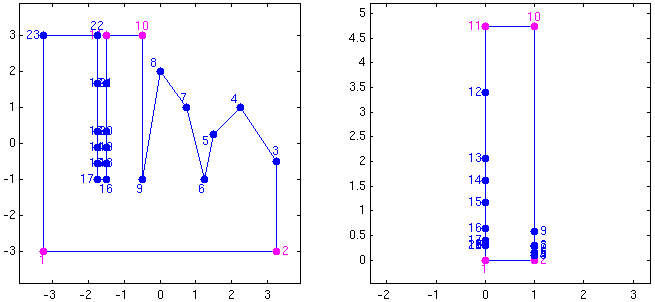
\includegraphics[width=2in]{figs-otherdomains/wigglytop2-bbox-numbered.png} \\
\caption{CRDT pic. EXPLAIN}
\label{wigglytop2-bbox-numbered}
% generated by Matlab
\end{figure}




\begin{table}[ht]
\begin{tabular}{c c c c c}\\
Method & Noise level & Sample size & MSE & se(MSE)\\
\hline
\hline
SC+TPRS & 0.02 & 1000 & 0.012993 & 0.0010068\\
TPRS & 0.02 & 1000 & 0.0022156 & 0.0003959\\
soap & 0.02 & 1000 & 0.0028811 & 0.011293\\
SC+TPRS & 0.005 & 1000 & 0.012856 & 0.0010157\\
TPRS & 0.005 & 1000 & 0.0021704 & 0.00039474\\
soap & 0.005 & 1000 & 0.0020087 & 0.0082462\\
SC+TPRS & 0.02 & 500 & 0.012305 & 0.0014609\\
TPRS & 0.02 & 500 & 0.0027819 & 0.00069713\\
soap & 0.02 & 500 & 0.11246 & 1.8866\\
SC+TPRS & 0.005 & 500 & 0.012316 & 0.0015265\\
TPRS & 0.005 & 500 & 0.0027275 & 0.00070468\\
soap & 0.005 & 500 & 0.38048 & 4.358\\
\end{tabular}
\caption{}
\label{example 4}
\end{table}

% boxplot
\begin{figure}[p]
\centering
% trim order l b r t
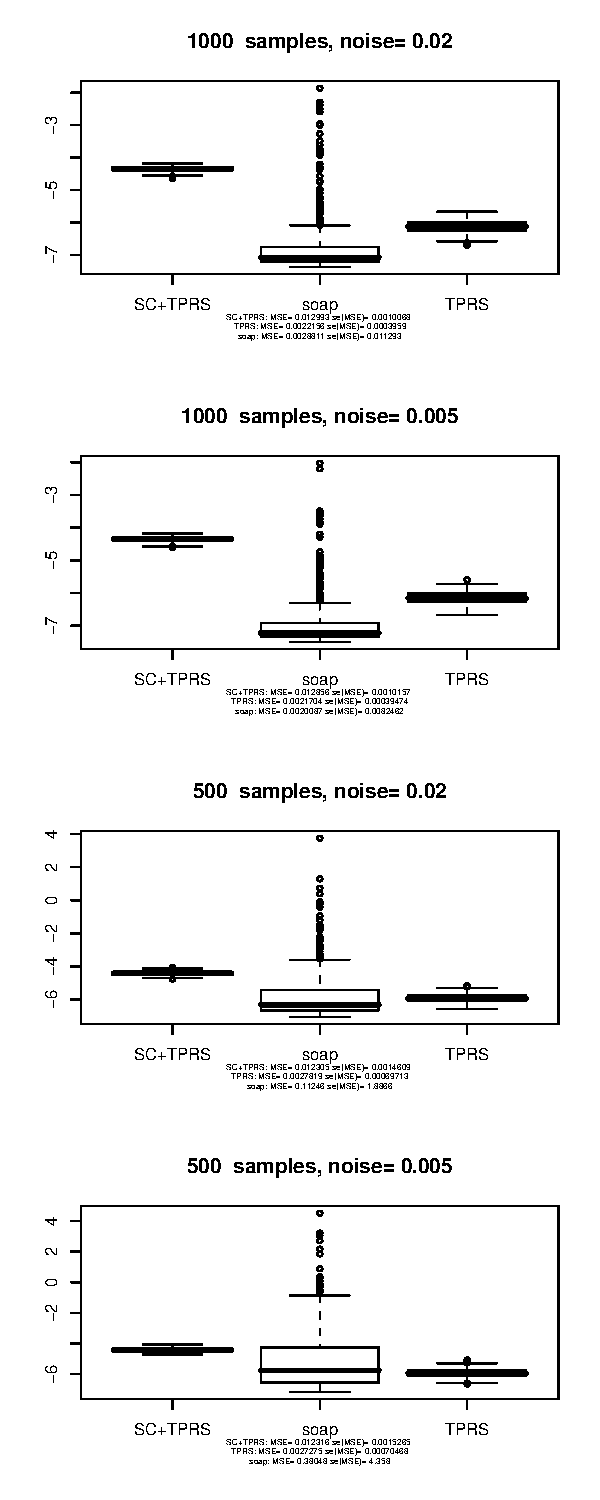
\includegraphics[width=3in]{figs-otherdomains/wigglytop2-bbox-boxplots.pdf} \\
\caption{Boxplot of mean squared error per prediction point over 500 replicates for the rectangle mapping for example 4.}
\label{wigglytop2-bbox-boxplots}
% generated by makeboxplots.R
\end{figure}


% realization
\begin{figure}
\centering
% trim order l b r t
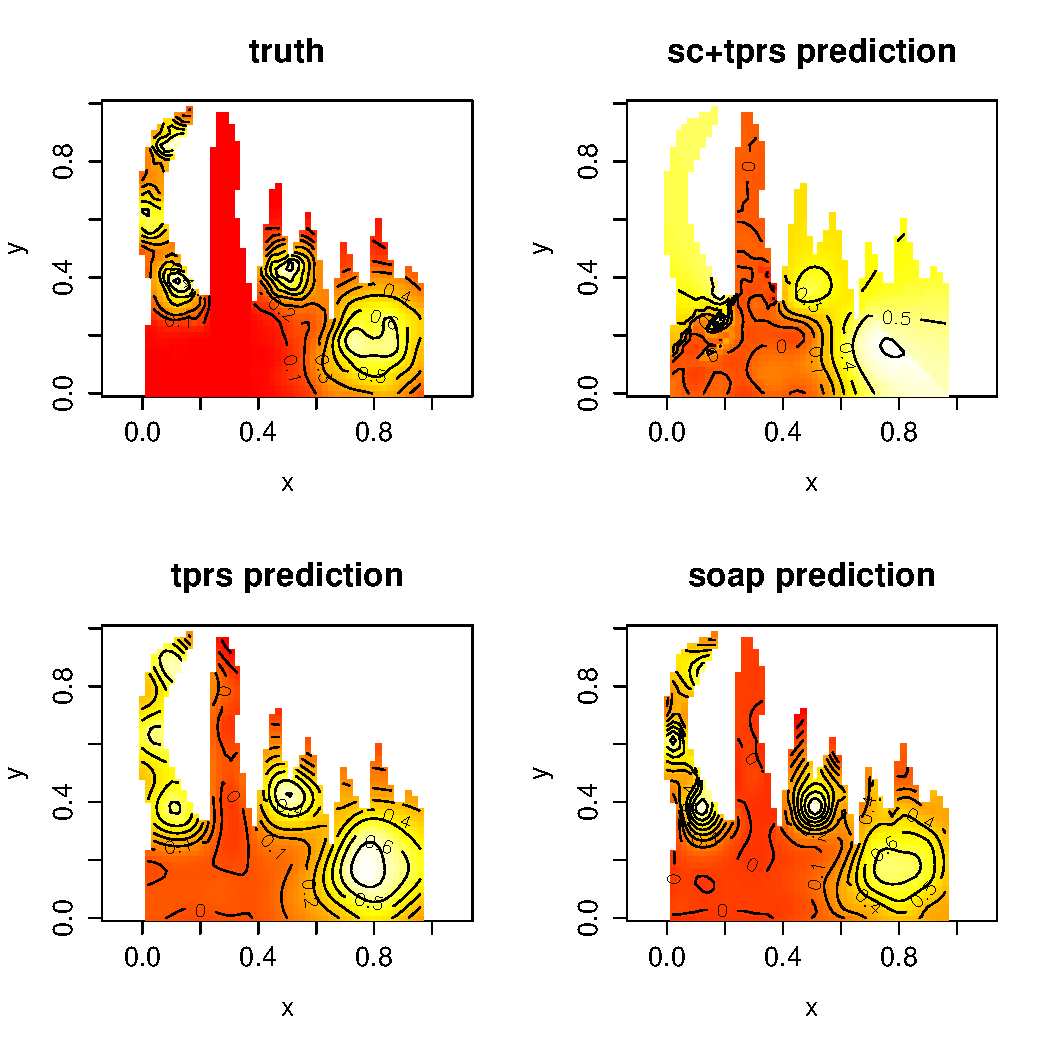
\includegraphics[width=3in]{figs-otherdomains/wigglytop2-bbox-real.pdf} \\
\caption{Truth and fits from one realization when there was a sample size of 500 and the noise level was set to 0.02 when the rectangular mapping was used for example 4.}
\label{wigglytop2-bbox-real}
% generated by wigglytop2-bbox fit.irregular.R
\end{figure}


\section{Conclusion}

This is rubbish.

Arbitrary vertex choice.

SQuashing of the features in wigglytop case.












\bibliographystyle{plainnat}
\bibliography{sc-refs}



\end{document}
